\documentclass[11pt, oneside]{article}   	% use "amsart" instead of "article" for AMSLaTeX format
\usepackage{geometry}                		% See geometry.pdf to learn the layout options. There are lots.
\geometry{letterpaper}                   		% ... or a4paper or a5paper or ... 
%\geometry{landscape}                		% Activate for for rotated page geometry
%\usepackage[parfill]{parskip}    		% Activate to begin paragraphs with an empty line rather than an indent
\usepackage{graphicx}				% Use pdf, png, jpg, or eps� with pdflatex; use eps in DVI mode
								% TeX will automatically convert eps --> pdf in pdflatex		
\usepackage{amssymb}
\usepackage{amsmath}
\usepackage{parskip}
\usepackage{color}
\usepackage{hyperref}

\title{Advanced techniques for Integrals}
%\author{The Author}
%\section{}
%\subsection*{}
\date{}							% Activate to display a given date or no date

\graphicspath{{/Users/telliott_admin/Dropbox/Tex/png/}}
% \begin{center} 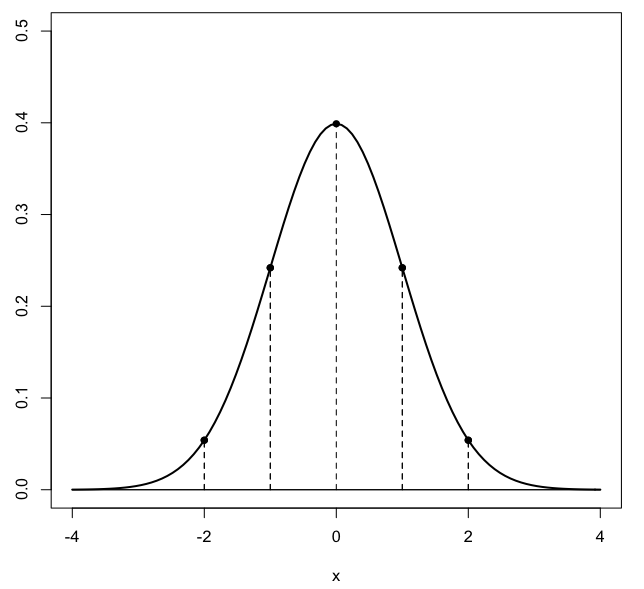
\includegraphics [scale=0.4] {gauss3.png} \end{center}
\begin{document}
\maketitle
\Large
Shankar has this example for the volume of a sphere of radius $R$.  We compute the volume for the part of the hemisphere that is in the first quadrant.  The surface is $f(x,y) = \sqrt{R^2 - x^2 - y^2}$ so the integral is
\[ \int_0^R \int_0^{\sqrt{R^2-y^2}} \sqrt{R^2 - x^2 - y^2} \ dx \ dy \]
There are several ways to approach this but what he does is an unusual trig substitution where the hypotenuse is $\sqrt{R^2 - y^2}$.  The substitution is 
\[ x = \sqrt{R^2 - y^2} \sin \theta \]
\[ dx =  \sqrt{R^2 - y^2} \cos \theta \ d \theta \]
(This integral is over the values of $x$ with $y$ \emph{fixed}, it may be treated as a constant.)  The integrand is
\[ \sqrt{R^2 - x^2 - y^2} = \sqrt{R^2 - y^2} \cos \theta \]

When $x=0 \rightarrow \theta=0$, and when $x=\sqrt{R^2 - y^2} \rightarrow \theta=\pi/2$ so the inner integral becomes
\[ \int_0^{\pi/2} \sqrt{R^2 - y^2} \cos \theta \sqrt{R^2 - y^2} \cos \theta \ d \theta \]
\[ R^2 - y^2 \int_0^{\pi/2} \cos^2 \theta \ d \theta \]
We've done this one many times.  One form of the answer is
\[ \frac{1}{2} ( \theta - \sin \theta \cos \theta) \]
For any interval involving $n \pi/2, n \in \{0,1,2 \dots\}$, the second term disappears.  So the result for $\theta = 0 \rightarrow \pi/2$ is just $\pi/4$.  

The outer integral becomes then
\[ \frac{\pi}{4} \int_0^R (R^2-y^2) \ dy \]
\[ = \frac{\pi}{4} (R^2 y - \frac{y^3}{3}) \bigg |_0^R =   \frac{\pi}{4} \  \frac{2}{3} R^3 \]
But there are eight such regions, so the total volume is
\[ 8\  \frac{\pi}{4} \   \frac{2}{3} R^3 = \frac{4}{3} \pi R^3 \]
The point of this example is that use of $\sqrt{R^2 - y^2}$ as the hypotenuse is useful and allowed because $y$ is constant, and it simplifies the bounds as well as the integral itself.

\subsection*{Gaussian integral}
We've worked this out elsewhere, but let's take a look at the following, called the Gaussian integral:
\[ \int_0^{\infty} e^{-ax^2} \ dx \]
Shankar calls this $I_0 (a)$, that is, it is a function of $a$:
\[ I_0(a) = \int_0^{\infty} e^{-ax^2} \ dx \]
and it is $I_0(a)$ because it is the zeroth version of a family of functions
\[ I_n(a) = \int_0^{\infty} x^n e^{-ax^2} \ dx \]

For the version
\[ I_0(a) = \int_0^{\infty} e^{-ax^2} \ dx \]
\[ 2 I_0(a) = \int_{-\infty}^{\infty} e^{-ax^2} \ dx \]
there is a special trick to convert this to polar coordinates
\[ 4 I_0(a)^2 = \int_{-\infty}^{\infty} e^{-ax^2} \ dx  \int_{-\infty}^{\infty} e^{-ay^2} \ dy  \]
Since the bounds of the $x$ and $y$ integrals are independent, as are the integrals themselves, we can turn this into the double integral
\[ = \int_{-\infty}^{\infty}  \int_{-\infty}^{\infty} e^{-ax^2} e^{-ay^2} \ dx \ dy  \]
\[ = \int_{-\infty}^{\infty}  \int_{-\infty}^{\infty} e^{-a(x^2 + y^2)} \ dx \ dy  \]
which can be converted to polar coordinates as
\[ = \int_{0}^{2 \pi}  \int_{-\infty}^{\infty} e^{-ar^2} \ r \ dr \ d \theta  \]
\[ = 2 \pi  \int_{0}^{\infty} e^{-ar^2} \ r \ dr   \]
\[ = 2 \pi \ (- \frac{1}{2a} ) \ (e^{-ar^2} \ \bigg |_{0}^{\infty} ) \]
At the upper limit we get $0$, and at the lower limit we get 
\[ e^{-\infty}  - e^{0} = 0 -1 = -1 \]
so the minus signs and the factors of two cancel and we have
\[ 4 I_0(a)^2 = \frac{\pi}{a}  \]
\[ I_0(a) = \frac{1}{2} \sqrt{\frac{\pi}{a}}  \]

For the rest of the family, the first one is easy
\[ I_1(a) = \int_0^{\infty} x e^{-ax^2} \ dx \]
\[ = -\frac{1}{2a} (e^{-ax^2} \ \bigg |_{0}^{\infty} ) = \frac{1}{2a}  \]
We get an approach to the second one in the following way.  Start with 
\[ I_0(a) = \int_0^{\infty} e^{-ax^2} \ dx \]
Differentiate with respect to $a$!
\[ \frac{d}{da} \int_0^{\infty} e^{-ax^2} \ dx = \int_0^{\infty} \frac{\partial}{\partial a} e^{-ax^2} \ dx  \]
\[ = \int_0^{\infty} -x^2 e^{-ax^2} \ dx  \]
For the left-hand side, we have
\[ \frac{d}{da} \ \frac{1}{2} \sqrt{\frac{\pi}{a}} = -\frac{\sqrt{\pi}}{4}  \frac{1}{a \sqrt{a}} = \frac{1}{4a} \sqrt{\frac{\pi}{a}} \] 
So finally
\[ \int_0^{\infty} x^2 e^{-ax^2} \ dx = \frac{1}{4a} \sqrt{\frac{\pi}{a}} \] 

\end{document}  